\documentclass[../report]{subfiles}
\setcounter{section}{0}
\begin{document}

本章では,本プロジェクトの目的及び活動概要について説明する.
\bunseki{堀沙枝香}

\section{目的} \label{sec:objective}
本グループは「認知症を予防すること」を大きな目的とし活動を進める.
そこで,1.3で挙げられた認知症と食習慣の関係に着目し,認知症になる前の段階の人(以下,対象者と記す)に向けて「食生活の改善をしてもらう」ことを目的に開発を行う.
そのため以下の内容により,食生活の見直しを促し,認知症予防を図ろうと考える.

\begin{itemize}
    \item 日々の食事を可視化し,蓄積された食事のデータを自身が閲覧する
    \item 他者から自身の食事に対するフィードバックを受ける
\end{itemize}

以上の内容を満たすため,本グループは「食生活を見直し認知症を予防するシステム,ふーろぐの開発」を行う.
具体的には,対象者に普段の食事を撮影し,写真というデータとして記録してもらう.
そのデータを自身閲覧,また対象者の家族や医療従事者に共有しメッセージを受け取ることができるシステムの開発を行う.
システムの流れは,まず高齢者でも簡単に撮影することができるように,本グループが作成するボックスに料理を置くだけで,自動的に写真の撮影ができる.
撮影した写真はテレビで閲覧することができる.
また,撮影した写真から栄養素を判断し,足りていない栄養を補えるような料理をテレビ画面から提案する.
一方で,対象者の家族や医療従事者は,Webから対象者が撮影した写真を閲覧することができる.
このとき,対象者が摂取した栄養素もチャート式で表示させる.
さらに,Web画面には対象者にメッセージを送信できる機能も加える.
メッセージが送信された場合には,対象者のテレビ画面にメッセージ内容が表示される.
これにより対象者は,自身の食生活に対するフィードバックを受け取ることができる.

これにより,対象者が食生活を簡単に記録でき,記録したデータを閲覧することができる.加えて,対象者は,他者からのフィードバックを受けることによって食生活の見直しができる.
また,医療従事者に記録したデータを提供することは,認知症になったときの意思決定支援に役立つと考える.
\bunseki{堀沙枝香}


\section{活動スケジュール}
プロジェクト全体の活動及び医療グループの活動スケジュールを以下に記す.

\begin{itemize}
    \item[] 5月
    \begin{itemize}
        \item 日々の食事を可視化し,蓄積された食事のデータを自身が閲覧する
        \item 他者から自身の食事に対するフィードバックを受ける
    \end{itemize}
\end{itemize}

以上の内容を満たすため,本グループは「食生活を見直し認知症を予防するシステム,ふーろぐの開発」を行う.
具体的には,対象者に普段の食事を撮影し,写真というデータとして記録してもらう.
そのデータを自身閲覧,また対象者の家族や医療従事者に共有しメッセージを受け取ることができるシステムの開発を行う.
システムの流れは,まず高齢者でも簡単に撮影することができるように,本グループが作成するボックスに料理を置くだけで,自動的に写真の撮影ができる.
撮影した写真はテレビで閲覧することができる.
また,撮影した写真から栄養素を判断し,足りていない栄養を補えるような料理をテレビ画面から提案する.
一方で,対象者の家族や医療従事者は,Webから対象者が撮影した写真を閲覧することができる.
このとき,対象者が摂取した栄養素もチャート式で表示させる.
さらに,Web画面には対象者にメッセージを送信できる機能も加える.
メッセージが送信された場合には,対象者のテレビ画面にメッセージ内容が表示される.
これにより対象者は,自身の食生活に対するフィードバックを受け取ることができる.

これにより,対象者が食生活を簡単に記録でき,記録したデータを閲覧することができる.加えて,対象者は,他者からのフィードバックを受けることによって食生活の見直しができる.
また,医療従事者に記録したデータを提供することは,認知症になったときの意思決定支援に役立つと考える.
\bunseki{堀沙枝香}


\section{活動スケジュール}
プロジェクト全体の活動及び医療グループの活動スケジュールを以下に記す.

\begin{itemize}
    \item[] 5月
    \begin{itemize}
        \item プロジェクト発足
        \item プロジェクトリーダー決定
        \item グループ分け
        \item グループリーダー決定
        \item キックオフイベント
        \item 南部先生によるフィールドワーク講座
        \item 認知症サポーター養成講座
        \item アイデアレビュー会
    \end{itemize}
    \item[] 6月
    \begin{itemize}
        \item 月例レビュー会
        \item 月例レビュー会の振り返り
        \item 石別フィールドワーク
        \item Skype会議
        \item ロボット開発ワークショップへの参加
        \item もの忘れカフェへの参加
        \item 中間成果発表ポスター作成開始
    \end{itemize}
    \item[] 7月
    \begin{itemize}
        \item 中間成果発表ポスターレビュー会
        \item 中間報告書作成開始
        \item 中間成果発表会
        \item 中間報告書提出
        \item 今後の活動についての話し合い
    \end{itemize}
    \item[] 8月
    \begin{itemize}
        \item 夏季休暇期間
    \end{itemize}
    \item[] 9月
    \begin{itemize}
        \item 今後の予定についての話し合い
        \item 仕様書の作成
        \item ユーザストーリーの作成
    \end{itemize}
    \item[] 10月
    \begin{itemize}
        \item プロジェクト活動のゴール決め
        \item 月例レビュー会
        \item 新しいフィールドについての話し合い
        \item 開発環境構築
        \item 「函館認知症の人を支える会」の人にシステム報告
        \item HAKODATEアカデミックリンク2017用ポスター作成開始
        \item もの忘れカフェへの参加とシステムについての説明
        \item システム体験準備開始
    \end{itemize}
    \item[] 11月
    \begin{itemize}
        \item 月例レビュー会
        \item HAKODATEアカデミックリンク2017
        \item もの忘れカフェにてシステム体験
        \item 最終成果発表会準備開始
        \item 最終成果発表会ポスター作成開始
    \end{itemize}
    \item[] 12月
    \begin{itemize}
        \item 最終成果発表会
        \item 最終報告書作成
    \end{itemize}
    \item[] 1月
    \begin{itemize}
        \item 最終報告書提出
    \end{itemize}
\end{itemize}
\bunseki{堀沙枝香}


\section{活動概要}
\subsection{学習とシステム案の検討} \label{sec:discuss}
認知症の症状やその療法,認知症に関する現状の社会問題や取り組みを本やインターネットを利用して個人で調べた.
そこで得た知識をもとに,個人でシステム案を検討し,それぞれの案をグループ内で共有した.案の内容については4.1 で述べる.
また,システム案の検討と同時に,既存の認知症に関するデバイスやアプリについても調べた.
\bunseki{堀沙枝香}

\subsection{認知症の人を支える会への提案}
「函館認知症の人を支える会」の人を大学にお招きし,認知症とは何か,認知症を引き起こす原因,中核症状と行動・心理症状,認知症の人の支援の仕方などといった内容の講座を開いて頂いた.
その後,本グループで考えているシステムを提案し,それについてディスカッション形式でご意見を頂いた.
頂いたご意見を参考にして,システム案の修正を行った.
頂いたご意見のについて詳しくは4.2.2 にて述べる.
\begin{figure}[htbp]
    \begin{center}
        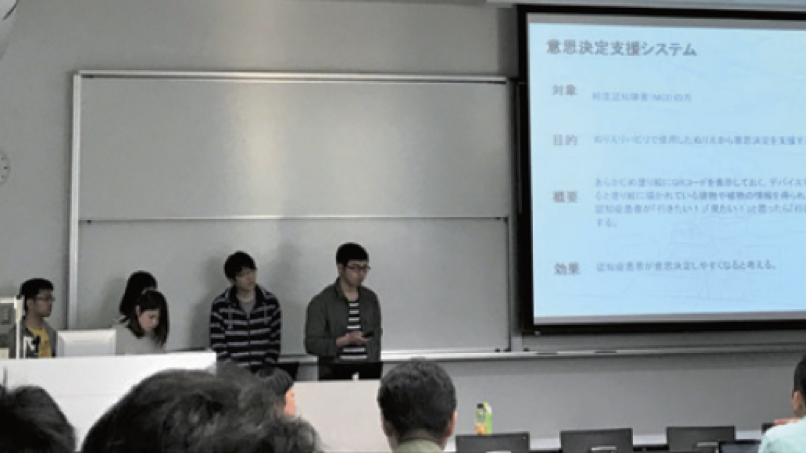
\includegraphics[width=10cm]{imgs/idea_review1.png}
        \caption{認知症サポーター養成講座}
    \end{center}
\end{figure}
\bunseki{堀沙枝香}

\subsection{認知症の臨床研究を行っている医師への提案}
実際の医療現場で認知症の人たちと関わっている京都府立医科大学の成本医師と,Skype を介して本グループで考えているシステムを提案し,一つ一つにご意見を頂いた.
頂いたご意見について詳しくは4.2.3 にて述べる.
その後,提案したシステム案の中で成本医師自身が気になったものを選んで頂き,その理由を伺った.
また,成本先生から事前に頂いていたキーワードの一つである「医療選択・意思決定支援」に必要としているものは何かを抽象的に尋ねた.
結果,医療従事者に提供される情報として望ましいものなど,今後システムを考える上で手がかりになるようなご意見を頂いた.
\begin{figure}[htbp]
    \begin{center}
        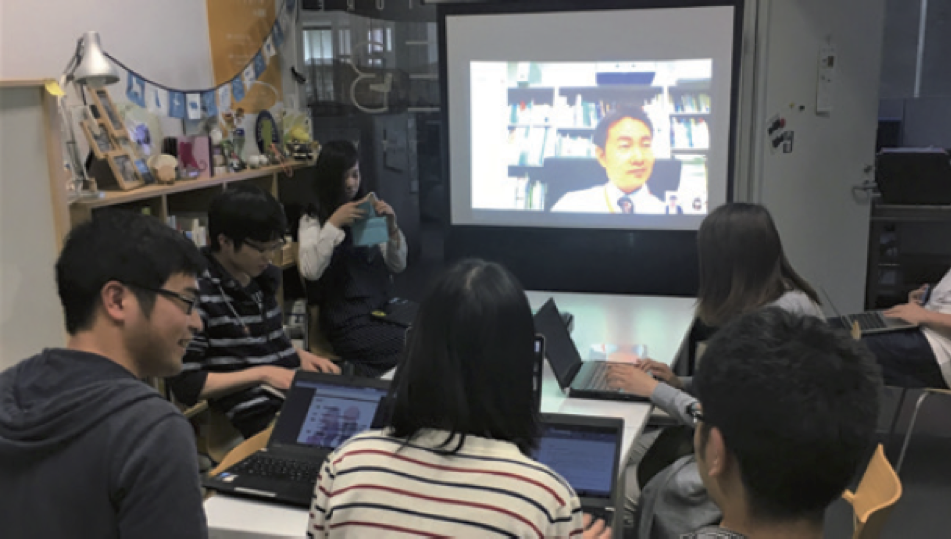
\includegraphics[width=10cm]{imgs/idea_review2.png}
        \caption{認知症サポーター養成講座}
    \end{center}
\end{figure}
\bunseki{堀沙枝香}

\subsection{もの忘れカフェへの提案} \label{sec:propose_cafe}
函館認知症の人を支える会の人が主催している,もの忘れカフェに参加した.
もの忘れカフェとは,月に一度,物忘れで困っている人やそんな人たちを支えたい人たちが集まり,話をする場である.
そこでの茶話会の時間を利用して,ボランティアの人に自己紹介も兼ねて,本グループの活動について紹介させて頂いた.
活動に興味を持ってくださったので,現状で考えているシステムについての説明をし,それについてご意見を頂いた.
頂いたご意見について詳しくは4.2.4 で述べる.
\bunseki{堀沙枝香}

\subsection{システム案の決定} \label{sec:decision}
\ref{sec:discuss}で生まれたシステム案修正に試行錯誤が続いたため,建設的なアイデアが生まれることを期待し,\ref{sec:discuss}で考えたシステム案とは全く違う目線で今までに得た学びを踏まえ,案の再検討を試みた.
結果「認知症になる前段階の人たちに食生活の見直しを促し,認知症予防を図ろう」といった方向性に決定し,「食生活を見直し認知症予防を図るシステム」を提案した.
\bunseki{堀沙枝香}

\subsection{中間成果発表会}
\ref{sec:decision}で提案したシステムや活動プロセスを,中間発表会でポスターセッション形式にて発表した.
発表の際に頂いたご意見をまとめた結果,「高齢者への撮影した写真データの見せ方」,「料理の撮影方法」などのシステム内容に改善の余地があると考えた.
本グループはこれらの方法に対し,検討を試みる及び改善することを今後の課題として追加する.
\bunseki{堀沙枝香}

\subsection{開発}
\ref{sec:objective}で挙げたシステムの開発を行うため,いくつかの実装を行った.
料理を自動で撮影するためのカメラの実装や,撮影した写真を閲覧するためのWebサーバの実装,また撮影した写真から栄養摂取量を摘出するため,料理画像認識の実装を行った.
詳しい実装方法については第6章にて述べる.
\bunseki{堀沙枝香}

\subsection{もの忘れカフェでの提案} \label{sec:propose_cafe2}
\ref{sec:propose_cafe}で紹介したもの忘れカフェに参加した.
\ref{sec:propose_cafe2}で説明したシステムから,\ref{sec:decision}で述べたシステムに変更したため,変更後のシステムについて主催者の人に報告した.
報告内容としては,現状考えているシステムの全体の流れについて説明した.
結果,着目点や発想については高く評価して頂いた.一方で,現状のシステムに足りていない,またユーザが求めている機能などを新たに発見することができた.
頂いた意見について詳しくは7.1.1で述べる.
\bunseki{堀沙枝香}

\subsection{HAKODATEアカデミックリンク2017}
\ref{sec:propose_cafe2}で報告した内容は,HAKODATEアカデミック2017でも,ポスターセッションと現段階のシステムを使用し,デモンストレーションを行いながら発表した.
デモンストレーションを行った際,システムを繰り返し何度も実行させているうちに,不必要な写真が撮影されてしまうなど,自動撮影処理が上手くいかなくなることが発生した.
このことから,撮影処理にあたるスクリプトの改善を行い,自動撮影処理の正確性を上げるよう検討した.
\bunseki{堀沙枝香}

\subsection{システム体験}
\ref{sec:propose_cafe}で紹介したもの忘れカフェに参加した.
今回は,主催者の人だけではなく,一般参加者の人にも本グループの開発するシステムを体験して頂くことを目的に参加した.
参加者にはまず,どのようなシステムであるかをよく理解して頂いた上で,システム体験のお願いをした.
具体的には,実際にシステムを使っている様子や説明を,理解しやすいよう寸劇を通して行い,興味を持って頂いた人に実際にシステムの体験をして頂いた.
体験後に頂いた意見について詳しくは7.1.2で述べる.
\begin{figure}[htbp]
    \begin{center}
        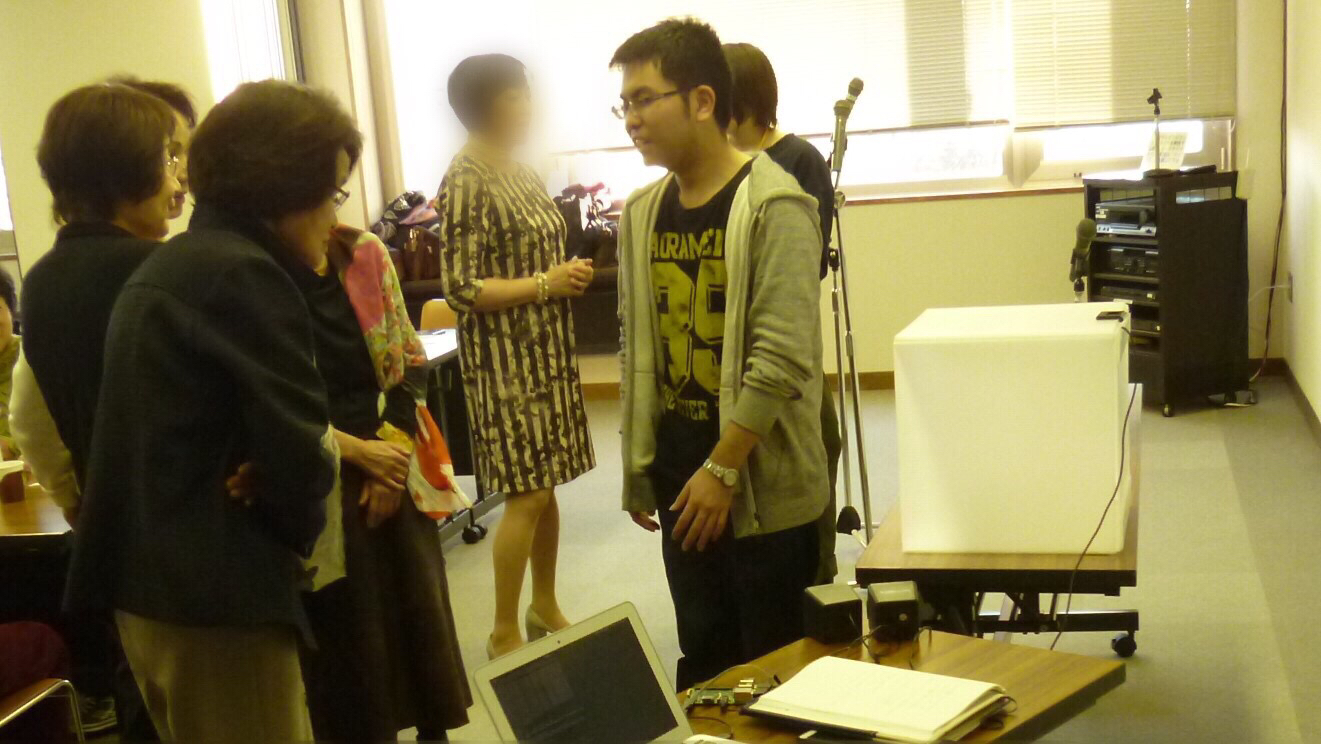
\includegraphics[width=10cm]{imgs/system_taiken.jpg}
        \caption{認知症サポーター養成講座}
    \end{center}
\end{figure}
\bunseki{堀沙枝香}

\end{document}
